\epigraph{By your words you will be justified, and by your words you will be condemned.}{Matthew 12:37.}
Conversation in the form of  languages has always been a trademark of humanity. 
It is one of the first skills that we humans acquire as kids, and never cease to use throughout our lives, whether 
 a person is ordering a burrito for lunch, taking classes, 
doing job interviews, discussing the result of an NHL game with friends, or even arguing with others. 
The significance of conversation/communication also transcends individuals: through conversations, humans can communicate a huge amount of information not only about
our surroundings (e.g., asking companions to watch out for the lions in the forest), but about ourselves (e.g., giving orders, talking about personal needs, etc). Such an ability leads to more effective social cooperation, and is a necessity for  
organizing a larger group of people (e.g., company, troop, etc). 

In the field of  artificial intelligence, attempts to imitate humans' ability to converse can be dated back to the early days of AI, and
this ability has long been 
associated with the general success of AI. 
In his epoch-making paper \cite{turing1950computing}, Alan Turing
proposed a method to test the general intelligence level of a machine, which is widely known as the Turing test or the Imitation game.
In the Turing test, 
 a machine is asked to 
talk with a human. The machine's intelligence level is decided by how well the machine is able to fool a human evaluator into believing that 
it, the machine, is a human based on its text responses. 
If the human evaluator cannot  tell the difference between the machine from a human, the machine is said to have passed the Turing test, which signifies a 
high level of intelligence of an AI.

Ever since the idea of the Turing test was proposed, various attempts have been proposed to pass the test. 
But we are still far from passing the test. 
In this section, we will briefly review the systems that have been proposed over the past decades.
Specifically, 
we will discuss 
three types of 
dialogue systems:  the chit-chat system, 
the frame-based goal oriented system, and
the interactive question-answering (QA) dialogue system. 
We will discuss the cases where they have been successfully applied, their pros and cons, and  why they are still not able to  pass the Turing test. 
The major focus of this thesis is about how to improve 
the chit-chat system and the interactive question-answering (QA) system. 

\section{A Brief Review of Existing Dialogue Systems}
\subsection{The Chit-chat Style System}
A chit-chat-oriented dialogue agent is designed to engage users, comfort them, provide mental support, or just chat with users whichever topic they want to talk about. 
The bot first needs to understand what its dialogue partner says, and then 
 generate meaningful and coherent responses based on this history.  
 Existing chit-chat systems mostly fall into the following three subcategories: the rule-based systems, the IR-based systems and the generation-based systems, as will be discussed in order below. 

\subsubsection{The Rule-based Systems}
Using rules is one of the most effective ways to generate dialogue utterances. 
Usually,
message inputs are first assessed  based on a set of pre-defined rules, e.g., 
a key-word look-up dictionary,
if-else conditions, or more sophisticated machine learning classifiers.
After rule conditions are evaluated, relevant actions will be executed, such as 
outputting an utterance in storage, manipulating the input message or selecting some related historical contexts. 


One of the most famous 
rule-based 
dialogue systems in history is  ELIZA \cite{weizenbaum1966eliza}. 
ELIZA operates by first searching a keyword existing in the input text from a real human
 based on a hand-crafted keyword dictionary. If a keyword is found, a rule is applied to 
 manipulate and
 transform the 
user's original input and forwarded back to the user. Otherwise, ELIZA responded either with a generic response or copying one sentence from the dialogue history.\footnote{\url{https://en.wikipedia.org/wiki/ELIZA}} 
 Extensions of ELIZA include PARRY \cite{parkinson1977conversational}, also described as "ELIZA with attitude",
which simulated a patient with schizophrenia. 
PARRY relies on global variables to keep track of the emotional state, as opposed to ELIZA where responses are generated only based on the previous sentence. 
A variety of chit-chat systems such as  Eugene Goostman,\footnote{\url{https://en.wikipedia.org/wiki/Eugene_Goostman}} 
Jabberwacky,\footnote{\url{https://en.wikipedia.org/wiki/Jabberwacky}} 
Cleverbot,\footnote{\url{https://en.wikipedia.org/wiki/Cleverbot}} 
Alice,\footnote{\url{https://en.wikipedia.org/wiki/Artificial_Linguistic_Internet_Computer_Entity}} 
AIML\footnote{\url{https://en.wikipedia.org/wiki/AIML}} were proposed after Eliza and PARRY. 

ELIZA-style systems are recognized as an important milestone in developing modern dialogue systems. 
More interestingly, 
 some of the systems seemed to be able to deceive some human evaluators to believe that they were talking with real people in a few specific scenarios \cite{thomas1995social,colby1972turing,pinar2000turing}.
 On the other hand, their drawbacks are obvious: 
Rule-based systems 
predominantly rely on
 the set of pre-defined rules.  
The number of these rules  skyrockets as the system gets more sophisticated;
Rule-based systems do not have the ability to understand human languages, nor do they know how to generate meaningful natural language utterances.
They are 
 thus only able to conduct very superficial conversations.  


\subsubsection{The IR-based Systems}
The IR-based methods  rely on information retrieval or nearest neighbor techniques  \cite{isbell2000cobot,jafarpour2010filter,yan2016learning,al2016conversational,yan2016docchat}.
Given a history input and a training corpus, the system copies a response from the training corpus.
The response selection process is usually
 based on the 
combination of the following
 two criteria: 
the history associated with the chosen response should be similar to the input dialogue history and the 
chosen response should be semantically related to the input dialogue history. 
Various ranking schemes such as semantic relatedness measurements (e.g., vector space models or TF-IDF), 
page-rank style relatedness propagation models, or personalization 
techniques
can be ensembled into a single ranking function 
and the response with the highest ranking score will be selected. 
The pros and cons of the IR-based models are both obvious: on one hand, the models are easy to implement relative to generation-based models;
responses are always grammatical (since responses are copied from the training set); and through the manipulation of 
the ranking function (e.g., adding rules, upweighing or downweighting some particular features), a developer has a relatively good (and direct) control on generating responses that he or she would like to see.\footnote{This is hardly true, or at least requires more human efforts in the generation-based system. One example is the generation-based system {\it Tay}, an artificial intelligence chatterbot via Twitter released by Microsoft, which posts inflammatory, offensive or even sexist and racist responses.} 
But on the other hand, the IR-based models lack the flexibility in handling the diversity of natural languages, the ability to handle important linguistic features such as 
context structure or coherence, 
and the capability of discerning 
 the subtle semantic difference between different input contexts. 
\subsubsection{The Generation-based Systems}
The generation-based system generates sentences token by token instead of  copying responses from the training set. The task can be formalized 
as an input-output mapping problem, where given the history dialogue utterances, the system needs to output a coherent and meaningful sequence of words.\footnote{Here, we refer to dialogue history, sources, inputs, stimulus,
and messages interchangeably, which all mean the dialogue history. We also refer to targets, outputs, and responses interchangeably, which mean the natural language utterance that the system needs to generate.}
The task was first studied by \newcite{ritter2011data},  who frame the response generation task as a
statistical machine translation (SMT) problem. The IBM-model \cite{brown1991aligning} is used  to learn the  word mapping rules between source  and target words (as shown in Figure \ref{IBM}) and the phrase-based MT model \cite{chiang2007hierarchical} is used for word decoding. The disadvantage of the MT-based system stems not only from the  complexity of the phrase-based MT model with many different components built separately, but also from the IBM model's intrinsic inflexibility in handling 
the 
implicit semantic and syntactic
relations between message-response pairs: unlike in MT, where there is usually a direct mapping between a word or phrase in the source sentence and another 
word or phrase
in the target sentence, 
in response generation, the  mapping is mostly beyond the word level, and 
 requires the semantic of the entire sentence. 
Due to this reason, the MT-based system is only good at handling the few cases in which word-level mapping is very clear as in Figure \ref{IBM}, but usually
fail to tackle
  the situations once the semantic of an input sentence gets  complex, sometimes outputting incoherent, or even ungrammatical responses. 
Furthermore, the MT-based system lacks the ability to leverage information in the multi-context situation. 

\begin{figure}
\center
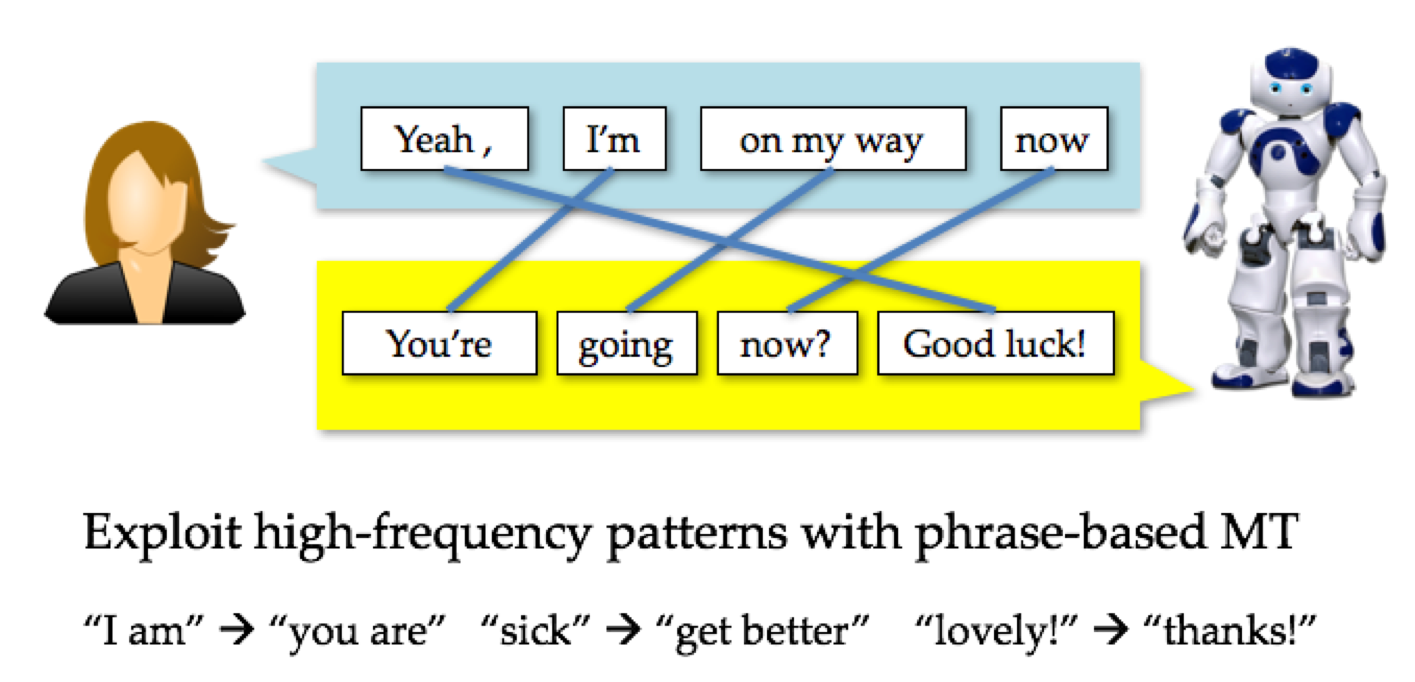
\includegraphics[width=4in]{img/michel.png}
\caption[Word alignments between   messages and responses using the IBM model]{Word alignments between   messages and responses using the IBM model. Image courtesy of Michel Galley.}
\label{IBM}
\end{figure}
Recent progress in SMT, which stems  from the use of neural 
language models \cite{mikolov2010recurrent,kalchbrenner2013recurrent,vaswani2013decoding} and neural sequence-to-sequence generation models (\sts) \cite{sutskever2014sequence,bahdanau2014neural,cho2014learning,luong2015effective,luong2014addressing,luong2016achieving}
have inspired a
variety of
attempts to extend neural
techniques to response generation \cite{sordoni2015neural,ghazvininejad2017knowledge,mostafazadeh2017image,serban2017hierarchical,serban2016building,serban2016generative,serban2017multiresolution}. 
Neural models offer the promise of scalability
and language-independence, together with the
capacity to implicitly learn semantic and syntactic
relations between pairs, and to capture contextual dependencies
in a way not possible
with conventional SMT approaches or IR-based approaches.

Due to these advantages, neural generation models are able generate more specific, coherent, and meaningful dialogue responses. 
On the other hand, 
a variety of important issues still remain unsolved: current  systems tend to generate plain and dull responses such as ``i don't know what you are talking about", which discourages the conversation; it is hard to endow a dialogue system with a consistent 
element of identity or persona (background facts or user
profile), language behavior or interaction style;
current systems usually focus on single-turn conversations, or two-turns at most, since
it is hard to give the system a long-term planning ability 
to conduct 
 multi-turn conversations that flow smoothly, coherently, and meaningfully.  
This thesis tries to address these issues. 



\subsection{The Frame-based  Dialogue Systems}
The frame-based system, first proposed by \newcite{bobrow1977gus}, models conversations  guided by frames, which represent the information at different 
levels within a conversation. 
For example, in a conversation about plane ticket booking, frames include 
important aspects such as 
{\it Person}, {\it Traveling Date}, 
{\it Destination}, {\it TimeRange of the flight}, etc. 
Frames of a conversation define the aspects that the conversation should cover and the relations (e.g., one frame is a prototype of another)
between frames
define how conversations should flow  \cite{walker1990mixed,seneff1992tina,chu1997tracking,san2001designing,seneff2002response}. 

  The simplest frame-based system is a finite-state machine, which asks the user a series of pre-defined questions based on the frames,
  and moves on to the next question
    if a customer provides an answer, and 
     ignores anything from the 
  customer if the response is not an answer. 
More complicated architectures
 allow the initiative of the conversation between the system and the user to shift at various points.
 These systems rely on a pre-defined frame and asks the user to fill slots in the frame, where a task is completed if all frame slots 
 have been filled . 
The limitation of the frame-based system is that the dialogue generation process is completely guided by what needs  to fill the slots. The system doesn't
have the ability to decide the progress
or the state
 of the conversation, e.g., whether the customer has rejected a suggestion, asked a question, or whether the system now needs to 
give suggestions or ask clarification questions, etc, and is thus not able to take a correct action given the progress so far.

To overcome these drawbacks, 
 more sophisticated state-based dialogue models \cite{nagata1994first,reithinger1996predicting,warnke1997integrated,stolcke2000dialogue,allen2001architecture} were designed. 
The \textsc{state-based dialogue system} is based on two key concepts, \textsc{dialogue state}, 
which denotes the progress of current conversation, including context information, intentions of the speakers, etc, 
and \textsc{dialogue acts}, which characterize the category of a dialogue utterance. 
The choice of a \textsc{dialogue act} is based on the \textsc{dialogue state} the conversation is currently in, and the key component of this system is to 
learn the optimal mapping between a state and an action to take, which is able  to maximize dialogue success.  
Reinforcement learning methods 
such as MDPs or POMDPs are widely used 
to learn such mappings based on external rewards that define dialogue success 
\cite{young2000probabilistic,young2002statistical,lemon2006isu,williams2007partially,young2010hidden,young2013pomdp}.
Recent advances in neural network models provide with more power and flexibility in keeping track of dialogue states and 
 modeling the mapping between the dialogue states and utterances to generate  \cite{wen2015semantically,mrkvsic2015multi,su2015learning,wen2016network,wen2016conditional,su2016continuously,su2016line,wen2017latent}. 

Frame-based systems have succeeded in a variety of applications such as booking flight tickets, reserving restaurants, etc, some of which have already been 
in use in our everyday life.  
The biggest advantages of frame-based system are that 
the goal of the system is explicitly defined and that the pre-defined frames give a very clear guidance on how a conversation should proceed.
On the other hand, its limitation is  clear:
 frame-based systems heavily rely on sophisticated  hand-crafted patterns or rules, and these rules are costly;
 rules have to be rebuilt when the system is adapted to a new domain or an old domain changes, making the system difficult to scale up. 
More broadly, 
it does not touch  the complex linguistic features involved in human conversations, such as context coherence, 
word usage (both semantic and syntactic), 
personalization, 
and  
are thus not able to capture the complexity and the intriguing nature of humans'
conversation. 

In this thesis, we do not focus on frame-based systems.

\subsection{The Question-Answering (QA) Based Dialogue System}
Another important dialogue system is the 
 factoid QA-based dialogue system, 
which is closely related to developing automated personal assistant systems such as Apple's Siri. 
A dialogue agent needs to answer customers' questions regarding different topics 
such as weather conditions, traffic congestion, news, stock prices, user schedules, retail prices, etc \cite{d1993personal,modi2005cmradar,myers2007intelligent,berry2011ptime}, either given a database of knowledge \cite{dodge2015evaluating,bordes2015large,weston2016dialog},
or from  texts \cite{hermann2015teaching,weston2015towards,weston2016dialog}.
The QA based dialogue system is thus related to a wide range of work in text-based or knowledge-base based question answering, e.g., \cite{hirschman2001natural,clarke2003passage,maybury2008new,berant2013semantic,iyyer2014neural,rajpurkar2016squad}  and many many others. 
The key difference between a QA-based dialogue system and a factoid QA-system is that 
the QA-based dialogue system is interactive \cite{rieser2009does}: instead of just having to answer one single question, 
the QA-based system needs the ability to handle a diverse category of interaction-related issues such as 
 asking for question clarification \cite{stoyanchev2013modelling,stoyanchev2014towards}, adapting answers given 
a human's feedback \cite{rieser2009does}, 
self-learning when encountering new questions or concepts
\cite{purver2006clarie}, etc.
To handle these issues, 
 the system needs to 
 take proper  actions based on the current conversation state, which resembles the key issue addressed in the \textsc{state-based dialogue system}. 

How a bot can 
be smart about interacting with humans, 
and how to improve itself through these interactions are not sufficiently studied. 
For example, asking for question clarification is only superficially touched in 
\newcite{stoyanchev2013modelling,stoyanchev2014towards} for cases where some important tokens are not well transcribed from the speech, for example,

A: {\it When did the problems with [power] start}?

B: {\it The problem with what}?

A: {\it Power}.

\noindent But  important scenarios such as what if  there is 
an out-of-vocabulary word in the original question,  how a bot can ask for hints, 
 and more importantly,  how a bot can 
be smart about deciding whether, when and what to ask  have rarely been studied. 
Another important aspect 
in developing interactive agent
that is missing from existing literature is that
a good  agent should have the
ability to learn from the online feedback: adapting its model when making mistakes
and reinforcing the model when a human's feedback is positive. This is particularly important
in the situation where the bot is initially trained in a supervised way on a fixed synthetic, domain-specific
or pre-built dataset before release, but will be exposed to a different environment after
release (e.g., more diverse natural language utterance usage when talking with real humans, different
distributions, special cases, etc.). 
There hasn't been any work discussing how a bot effectively improve itself from online feedback by accommodating various feedback signals.  
This thesis tries to address these questions. 


\section{Thesis Outline}
In this dissertation, we mainly address problems involved in the  
chit-chat system and the interactive QA system. 
First, we explore how to build an engaging chit-chat style dialogue system that is able to conduct 
interesting, meaningful, coherent, consistent, and long-term conversation with humans.  
More specially, 
for the chit-chat system,
we (a) use mutual information to avoid dull and generic responses
\cite{li2015diversity,li2016simple,li2017learning}; (b) address user consistency issues to avoid inconsistent responses from the same user \cite{li2016persona}; (c) develop reinforcement learning 
methods to foster the long-term success of conversations \cite{li2016deep}; and (d) use adversarial learning methods to generate machine responses that are indistinguishable from human-generated responses \cite{li2017adversarial}; 

Second, we explore how a bot can best improve itself through the online interactions with humans that makes a
chatbot system trully \textsc{interactive}. 
We  
develop interactive dialogue  systems for factoid question-answering: 
(a)  we
design an environment that provides the agent the ability to ask humans questions  and to learn when and what to ask \cite{li2016learning};
(b) we train a conversation agent through interaction with humans in an
online fashion, where a bot improves through communicating with humans and learning from the mistakes
that it makes \cite{li2016dialogue}. 

We start off by providing background knowledge on \sts models, memory network models and policy gradient reinforcement learning models in Chapter 2. 
The aforementioned four problems for the
chit-chat style
 dialogue generation systems will be detailed in Chapters 3,4,5,6,
 and the two issues with the interactive QA system will be detailed in Chapters 7 and 8. 
 We conclude this dissertation and discuss future avenue for chatbot development in Chapter 9.
 
 
\subsection{Open-Domain Dialogue Generation}
\subsubsection*{Mutual Information to Avoid Generic Responses} 
An engaging response generation system should be able to output grammatical, coherent responses that are diverse and interesting.
In practice, however,  neural conversation models exhibit a tendency to generate dull, trivial or non-committal responses, often involving high-frequency phrases along the lines of \textit{I~don't know} or  \textit{I'm OK} \cite{sordoni2015neural,serban2015hierarchical,vinyals2015neural}. 
This behavior is ascribed to the relative frequency of generic responses like 
 \textit{I don't know} in conversational datasets, in contrast with the relative sparsity of other, more contentful or specific alternative responses.
 It appears that by optimizing for the likelihood of outputs/targets/responses given inputs/sources/messages, 
neural models assign high probability to ``safe'' responses. 
The question is how to overcome the neural models' predilection for the commonplace. Intuitively, we want to capture not only the dependency of responses on messages, but also the inverse, the likelihood that a message will be provided to a given response. Whereas the sequence  \textit{I don't know} is of high probability in response to most question-related messages, the reverse will generally not be true, since \textit{I don't know}  can be a response to everything, making it hard to guess the original input question. 

We propose to capture this intuition by using Maximum Mutual Information (MMI), as an optimization objective that measures the mutual dependence between inputs and outputs, as opposed to 
the uni-directional dependency from sources to targets in the traditional MLE objective function.
We present practical training and decoding strategies for neural generation models that use MMI as objective function.
We demonstrate that using MMI results in a clear decrease in the proportion of generic response sequences, and 
find a significant performance boost from the proposed models as measured by  BLEU \cite{papineni2002bleu} and human evaluation.
{\it This chapter is based on the following three papers: \cite{li2015diversity,li2016simple,li2017learning}, and will be detailed in Section 3}. 

\subsubsection*{Addressing the Speaker Consistency Issue} 
An issue that stands out with current dialogue systems is the lack of speaker consistency: if a human asks a bot a few questions, there is no guarantee that answers from the bot are consistent. 
This is because 
responses are selected based on likelihood assigned by the pre-trained model, which does not have the ability to model speaker consistency. 

In \newcite{li2016persona}, we address the challenge of consistency and how to endow data-driven systems with the coherent ``persona'' needed to model human-like behavior, whether as personal assistants, personalized avatar-like agents, or game characters.\footnote{\cite{vinyals2015neural} suggest that the lack of a coherent personality makes it impossible for current systems to pass the Turing test.} 
For present purposes, we will define \textsc{persona} as the character that an artificial agent, as actor, plays or performs during conversational interactions.
A~persona can be viewed as a composite of elements of identity (background facts or user profile), language behavior, and interaction style. 
A persona is also adaptive, since an agent may need to present different facets to different human interlocutors depending on the demands of the interaction. 
We 
 incorporate personas as embeddings and explore two persona models, a single-speaker \textsc{Speaker Model} and a dyadic \textsc{Speaker-Addressee Model}, within the \sts framework. 
The Speaker Model integrates a speaker-level vector representation into the target part of the \sts model.
Analogously, the Speaker-Addressee model encodes the interaction patterns of two interlocutors by constructing an interaction representation from their individual embeddings and incorporating it into the \sts model. 
These persona vectors are trained on human-human conversation data and used at test time to generate personalized responses.
Our experiments on an open-domain corpus of Twitter conversations and dialog datasets comprising TV series scripts show that leveraging persona vectors can improve relative performance up to $20\%$ in BLEU score and $12\%$ in perplexity, with a commensurate gain in consistency as judged by human annotators. 
{\it This chapter is based on the following paper: \newcite{li2016persona}, and will be detailed in Section 4}. 


\subsubsection*{Fostering Long-term Dialogue Success}
Current dialogue generation models are trained by predicting the next {\bf single} dialogue turn in a given conversational context using the maximum-likelihood estimation (MLE) objective function. 
However, this does not mimic how we humans talk. In everyday conversations from a human, each human dialogue episode consists tens of, or even hundreds of dialogue turns rather than only one turn; humans are
smart in controlling the informational flow in a conversation for the long-term success of the conversation. 
Current models' incapability of handling this long-term success result in repetitive and generic responses.\footnote{The fact that current models tend to generate highly generic responses such as``{\it I don't know}" regardless of the input \cite{sordoni2015neural,serban2015hierarchical,li2015diversity} can be ascribed to the model's incapability of handling long-term dialogue success:
apparently {\it ``I don't know"} is not a good action to take, since it closes the conversation down} 

We need a conversation framework that has the ability to (1)  integrate developer-defined rewards that better mimic the true goal of chatbot development
  and (2)  model the long-term influence of a generated response in an ongoing dialogue.
To achieve these goals,  we draw on the insights of reinforcement learning, which
have been widely applied in MDP and POMDP dialogue systems.
We introduce a neural reinforcement learning (RL) generation method, 
which can optimize long-term rewards designed by system developers.
Our model uses the encoder-decoder architecture as its backbone, and 
 simulates conversation between two virtual agents to explore the space of possible actions while learning to maximize expected reward.
We define simple heuristic approximations to rewards that characterize
 good conversations: good conversations are forward-looking \cite{All92} or interactive (a turn suggests
 a following turn), informative, and coherent.
  The parameters of an encoder-decoder RNN define a policy over an infinite action space consisting of all possible utterances.
  The agent learns a policy by optimizing the long-term developer-defined reward from ongoing dialogue simulations using policy gradient methods \cite{williams1992simple},
  rather than the MLE objective defined in standard \sts models. 

Our model thus integrates the power of \sts systems to learn compositional semantic
meanings of utterances with the strengths of reinforcement learning in
optimizing for long-term goals across a conversation.
 Experimental results  demonstrate that our approach fosters a more sustained dialogue and
  manages to produce more interactive  responses than standard \sts models trained using the MLE objective.
  {\it This chapter is based on the following paper: \newcite{li2016deep}, and will be detailed in Section 5}. 

  
  \subsubsection*{Adversarial Learning for Dialogue Generation}
  Open domain dialogue generation  aims at generating meaningful and
coherent dialogue responses given input dialogue
history. 
   Current  systems   
   approximate such a goal 
   using imitation learning or variations of imitation learning: 
    predicting the
next dialogue utterance in human conversations
given the dialogue history. 
 Despite its success, many
issues emerge resulting from this over-simplified
training objective: responses are highly dull and
generic,  repetitive, and short-sighted. 
   



Solutions to these problems require answering a few fundamental questions: 
what are the crucial aspects that define an ideal conversation, how can we quantitatively measure them, and how can we incorporate them into 
a machine learning system:
A good dialogue model should generate utterances indistinguishable from human dialogues.
Such a goal suggests a training objective 
resembling the idea of the Turing test \cite{turing1950computing}.
We borrow the idea of adversarial training \cite{goodfellow2014generative} in 
computer
vision, in which we jointly train two models, 
a generator (which takes the form of the neural  \sts model) that defines the probability of generating a dialogue sequence, and 
a discriminator
that labels dialogues as human-generated or machine-generated. 
This discriminator  is analogous to  the evaluator in the Turing test.
We cast the task as a reinforcement learning problem, in which the quality of machine-generated utterances is measured by its ability to fool the discriminator into believing that it is a human-generated one. The output from the discriminator is used as a reward to the generator, pushing it to generate 
utterances indistinguishable from human-generated dialogues. 

Experimental results demonstrate that our approach
produces more interactive, interesting, and
non-repetitive responses than standard SEQ2SEQ
models trained using the MLE objective function.
  {\it This chapter is based on the following paper: \newcite{li2017adversarial}, and will be detailed in Section 6}. 
\subsection{Building Interactive Bots for Factoid Question-Answering}

  \subsubsection*{Learning by  Asking Questions}
  For current chatbot systems, when the bot encounters a confusing situation such as an unknown surface form (phrase
or structure), a semantically complicated sentence or an unknown word, the agent will either make
a (usually poor) guess or will redirect the user to other resources (e.g., a search engine, as in Siri).
Humans, in contrast, can adapt to many situations by asking questions: when a student is asked a question by a teacher, but is not confident about the answer, they may ask
for clarification or hints. A good conversational agent should have this ability
to interact with a customer. 

Here, we try to bridge the gap between how a human and an end-to-end machine learning system by equipping the bot with the ability to ask questions.
We identify three categories of mistakes a bot can make during dialogue
: (1) the bot has
problems understanding the surface form of the text of the dialogue partner, e.g., the phrasing of
a question; (2) the bot has a problem with reasoning, e.g., it fails to retrieve and connect the
relevant knowledge to the question at hand; (3) the bot lacks the knowledge necessary to answer
the question in the first place -- that is, the knowledge sources the bot has access to do not contain
the needed information.
All the situations above can be potentially addressed through interaction with the dialogue partner.
Such interactions can be used to learn to perform better in future dialogues. If a human bot has
problems understanding a teacher's question, they might ask the teacher to clarify the question. If
the bot doesn't know where to start, they might ask the teacher to point out which known facts
are most relevant. If the bot doesn't know the information needed at all, they might ask the
teacher to tell them the knowledge they're missing, writing it down for future use.

We explore how
a bot can benefit from interaction by asking questions in both offline supervised settings and online
reinforcement learning settings, as well as how to choose when to ask questions in the latter setting.
In both cases, we find that the learning system improves through interacting with users.
{\it This chapter is based on the following paper: \newcite{li2016learning}, and will be detailed in Section 7}. 

   \subsubsection*{Dialogue Learning with Human-in-the-Loop}
  A good conversational agent  
should have the ability to learn from the online feedback from a teacher: adapting its model when making mistakes and reinforcing the model when the teacher's feedback is positive.
This is particularly important in the situation where the bot is initially trained in a supervised way on a fixed synthetic, domain-specific or pre-built dataset before release, but will be exposed to
a different environment after release
 (e.g.,
 more diverse natural language utterance usage when talking with real humans, different distributions, special cases, etc.).  Most recent research
has focused on training a bot
from fixed training sets of labeled data but seldom on how the bot can
improve through online interaction with humans.
Human (rather than machine) language learning happens during communication \citep{bassiri2011interactional,werts1995instructive},
and not from labeled datasets, hence making this an important subject to study.


Here, we explore this direction by
 training a bot through interaction with teachers in an online fashion.
 The task is formalized under the general framework of reinforcement learning
via the teacher's (dialogue partner's) feedback to the dialogue actions from the bot.
 The dialogue takes place in the context of question-answering tasks and the bot has to, given either a short story or a set of facts, answer a set of questions from the teacher.
We consider two types of feedback: explicit numerical rewards as in conventional
reinforcement learning, and textual feedback which is more natural in human dialogue, following
\citep{weston2016dialog}.
We consider two online training scenarios:
(i) where the task is built with a dialogue simulator allowing for easy analysis and repeatability
of experiments; and (ii) where the teachers are real humans using Amazon Mechanical Turk.

    We explore  important issues involved in online learning
   such as  how a bot can be most efficiently trained using a minimal amount of teacher's feedback,
 how a bot can harness different types of feedback signal,
how to avoid pitfalls such as instability during online learing with different types of feedback via
 data balancing and exploration,
and how to make learning with real humans feasible via data batching.
Our findings indicate that
it is feasible to build a pipeline
that starts from a model trained with fixed data and then learns from interactions with humans
to improve itself. 
{\it This chapter is based on the following paper: \newcite{li2016dialogue}, and will be detailed in Section 8}. 

 

